%\documentclass[fleqn]{book}
\documentclass[11pt]{amsbook}

\usepackage[turkish]{babel}

%\usepackage{../HBSuerDemir}	% ------------------------
\usepackage{../Ceyhun}	% ------------------------
\usepackage{../amsTurkish}


\begin{document}
% ++++++++++++++++++++++++++++++++++++++
\hPage{102}
% ++++++++++++++++++++++++++++++++++++++
Bu tanımlardan,
 \[
	Ç(d,a)_{+1} = Ç(d,a)\\
 \]

ve genellikle,
    
\[
	A^n \text{ \{ } Ç(d,a) \text{ \} }  \neq A \text{ \{ } Ç(d,a)_{+n} \text{ \}\\ } 
\]
   
olduğu gözden kaçmamalıdır. Şekil 2.7.3 de ayrıt ve katkılı ayrıt çizgelerine örnekler verilmiştir.\\

\begin{center}
	\begin{tabular}{cccc}
		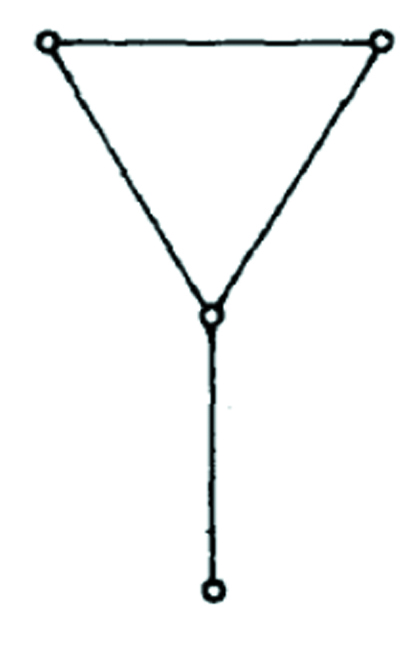
\includegraphics[width=0.2\textwidth]{images/1}
		&
		\quad 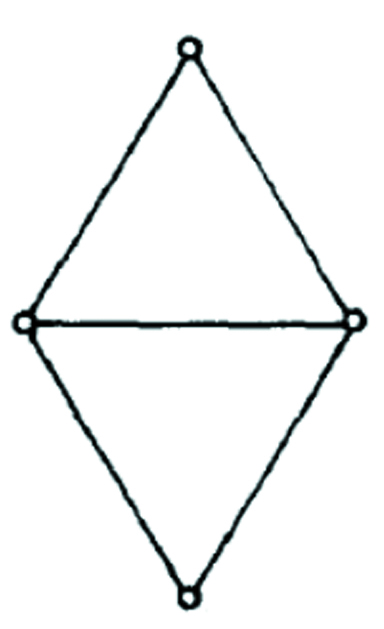
\includegraphics[width=0.195\textwidth]{images/2}
		&
		\quad 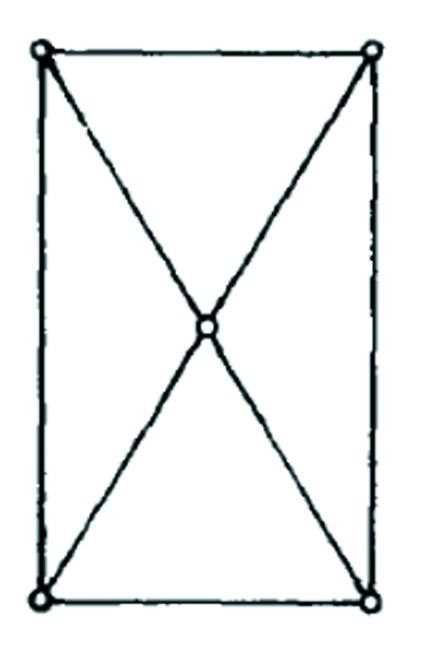
\includegraphics[width=0.21\textwidth]{images/3}
		&
		\quad 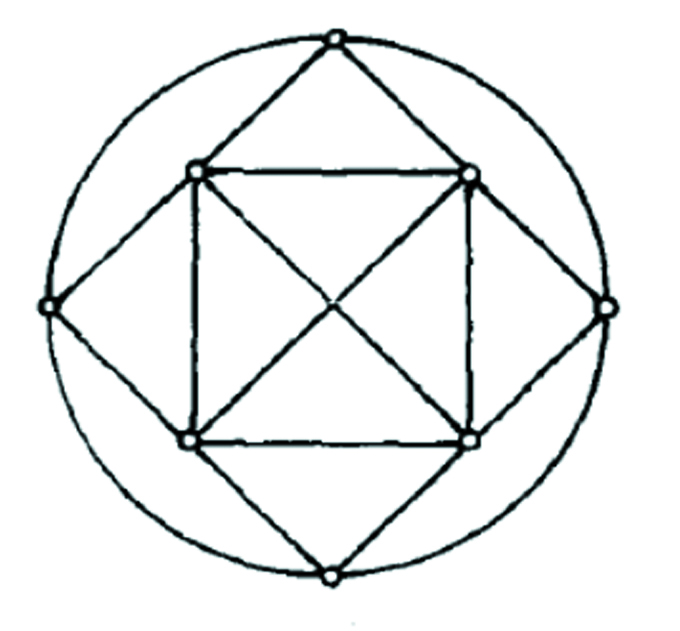
\includegraphics[width=0.34\textwidth]{images/4}\\

		Ç
		&
		\quad A$\{Ç\}$
		&
		\quad $A^2 \{Ç\}$
		&
		\quad $A^3 \{Ç\}$ \\
	\end{tabular}
\end{center}

\begin{center}
	(a)
\end{center}

\begin{center}
	\begin{tabular}{cc}
		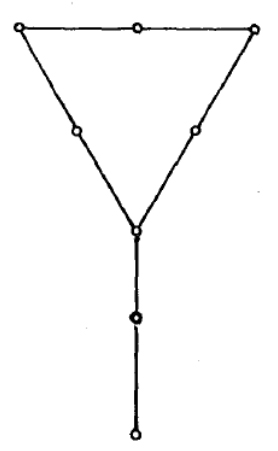
\includegraphics[width=0.3\textwidth]{images/5}
		&
		\quad 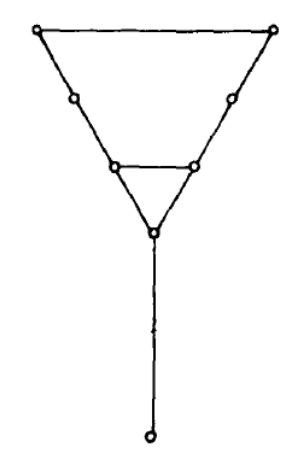
\includegraphics[width=0.32\textwidth]{images/6}\\

		$Ç_{+2}$
		&
		\quad A $\{Ç_{+2}\}$
	\end{tabular}
\end{center}

\begin{center}
	(b)
\end{center}

\end{document}